\documentclass{ws-ijseke}

\makeatletter
\@ifundefined{lhs2tex.lhs2tex.sty.read}  {\@namedef{lhs2tex.lhs2tex.sty.read}{}  \newcommand\SkipToFmtEnd{}  \newcommand\EndFmtInput{}  \long\def\SkipToFmtEnd#1\EndFmtInput{}  }\SkipToFmtEnd

\newcommand\ReadOnlyOnce[1]{\@ifundefined{#1}{\@namedef{#1}{}}\SkipToFmtEnd}
\usepackage{amstext}
\usepackage{amssymb}
\usepackage{stmaryrd}
\DeclareFontFamily{OT1}{cmtex}{}
\DeclareFontShape{OT1}{cmtex}{m}{n}
  {<5><6><7><8>cmtex8
  <9>cmtex9
  <10><10.95><12><14.4><17.28><20.74><24.88>cmtex10}{}
\DeclareFontShape{OT1}{cmtex}{m}{it}
  {<-> ssub * cmtt/m/it}{}
\newcommand{\texfamily}{\fontfamily{cmtex}\selectfont}
\DeclareFontShape{OT1}{cmtt}{bx}{n}
  {<5><6><7><8>cmtt8
  <9>cmbtt9
  <10><10.95><12><14.4><17.28><20.74><24.88>cmbtt10}{}
\DeclareFontShape{OT1}{cmtex}{bx}{n}
  {<-> ssub * cmtt/bx/n}{}
\newcommand{\tex}[1]{\text{\texfamily#1}}	
\newcommand{\Sp}{\hskip.33334em\relax}


\newcommand{\Conid}[1]{\mathit{#1}}
\newcommand{\Varid}[1]{\mathit{#1}}
\newcommand{\anonymous}{\kern0.06em \vbox{\hrule\@width.5em}}
\newcommand{\plus}{\mathbin{+\!\!\!+}}
\newcommand{\bind}{\mathbin{>\!\!\!>\mkern-6.7mu=}}
\newcommand{\rbind}{\mathbin{=\mkern-6.7mu<\!\!\!<}}\newcommand{\sequ}{\mathbin{>\!\!\!>}}
\renewcommand{\leq}{\leqslant}
\renewcommand{\geq}{\geqslant}
\usepackage{polytable}

\@ifundefined{mathindent}  {\newdimen\mathindent\mathindent\leftmargini}  {}
\def\resethooks{  \global\let\SaveRestoreHook\empty
  \global\let\ColumnHook\empty}
\newcommand*{\savecolumns}[1][default]  {\g@addto@macro\SaveRestoreHook{\savecolumns[#1]}}
\newcommand*{\restorecolumns}[1][default]  {\g@addto@macro\SaveRestoreHook{\restorecolumns[#1]}}
\newcommand*{\aligncolumn}[2]  {\g@addto@macro\ColumnHook{\column{#1}{#2}}}

\resethooks

\newcommand{\onelinecommentchars}{\quad-{}- }
\newcommand{\commentbeginchars}{\enskip\{-}
\newcommand{\commentendchars}{-\}\enskip}

\newcommand{\visiblecomments}{  \let\onelinecomment=\onelinecommentchars
  \let\commentbegin=\commentbeginchars
  \let\commentend=\commentendchars}

\newcommand{\invisiblecomments}{  \let\onelinecomment=\empty
  \let\commentbegin=\empty
  \let\commentend=\empty}

\visiblecomments

\newlength{\blanklineskip}
\setlength{\blanklineskip}{0.66084ex}

\newcommand{\hsindent}[1]{\quad}\let\hspre\empty
\let\hspost\empty
\newcommand{\NB}{\textbf{NB}}
\newcommand{\Todo}[1]{$\langle$\textbf{To do:}~#1$\rangle$}

\EndFmtInput
\makeatother
\ReadOnlyOnce{polycode.fmt}\makeatletter

\newcommand{\hsnewpar}[1]  {{\parskip=0pt\parindent=0pt\par\vskip #1\noindent}}

\newcommand{\hscodestyle}{}


\newcommand{\sethscode}[1]  {\expandafter\let\expandafter\hscode\csname #1\endcsname
  \expandafter\let\expandafter\endhscode\csname end#1\endcsname}


\newenvironment{compathscode}  {\par\noindent
  \advance\leftskip\mathindent
  \hscodestyle
  \let\\=\@normalcr
  \let\hspre\(\let\hspost\)  \pboxed}  {\endpboxed\)  \par\noindent
  \ignorespacesafterend}

\newcommand{\compaths}{\sethscode{compathscode}}


\newenvironment{plainhscode}  {\hsnewpar\abovedisplayskip
  \advance\leftskip\mathindent
  \hscodestyle
  \let\hspre\(\let\hspost\)  \pboxed}  {\endpboxed  \hsnewpar\belowdisplayskip
  \ignorespacesafterend}

\newenvironment{oldplainhscode}  {\hsnewpar\abovedisplayskip
  \advance\leftskip\mathindent
  \hscodestyle
  \let\\=\@normalcr
  \(\pboxed}  {\endpboxed\)  \hsnewpar\belowdisplayskip
  \ignorespacesafterend}


\newcommand{\plainhs}{\sethscode{plainhscode}}
\newcommand{\oldplainhs}{\sethscode{oldplainhscode}}
\plainhs


\newenvironment{arrayhscode}  {\hsnewpar\abovedisplayskip
  \advance\leftskip\mathindent
  \hscodestyle
  \let\\=\@normalcr
  \(\parray}  {\endparray\)  \hsnewpar\belowdisplayskip
  \ignorespacesafterend}

\newcommand{\arrayhs}{\sethscode{arrayhscode}}


\newenvironment{mathhscode}  {\parray}{\endparray}

\newcommand{\mathhs}{\sethscode{mathhscode}}


\newenvironment{texthscode}  {\(\parray}{\endparray\)}

\newcommand{\texths}{\sethscode{texthscode}}


\def\codeframewidth{\arrayrulewidth}
\RequirePackage{calc}

\newenvironment{framedhscode}  {\parskip=\abovedisplayskip\par\noindent
  \hscodestyle
  \arrayrulewidth=\codeframewidth
  \tabular{@{}|p{\linewidth-2\arraycolsep-2\arrayrulewidth-2pt}|@{}}  \hline\framedhslinecorrect\\{-1.5ex}  \let\endoflinesave=\\
  \let\\=\@normalcr
  \(\pboxed}  {\endpboxed\)  \framedhslinecorrect\endoflinesave{.5ex}\hline
  \endtabular
  \parskip=\belowdisplayskip\par\noindent
  \ignorespacesafterend}

\newcommand{\framedhslinecorrect}[2]  {#1[#2]}

\newcommand{\framedhs}{\sethscode{framedhscode}}


\newenvironment{inlinehscode}  {\(\def\column##1##2{}  \let\>\undefined\let\<\undefined\let\\\undefined
  \newcommand\>[1][]{}\newcommand\<[1][]{}\newcommand\\[1][]{}  \def\fromto##1##2##3{##3}  \def\nextline{}}{\) }
\newcommand{\inlinehs}{\sethscode{inlinehscode}}


\newenvironment{joincode}  {\let\orighscode=\hscode
  \let\origendhscode=\endhscode
  \def\endhscode{\def\hscode{\endgroup\def\@currenvir{hscode}\\}\begingroup}
    \orighscode\def\hscode{\endgroup\def\@currenvir{hscode}}}  {\origendhscode
  \global\let\hscode=\orighscode
  \global\let\endhscode=\origendhscode}
\makeatother
\EndFmtInput

\usepackage{siunitx}

\usepackage{multirow}
\usepackage{amssymb}
\setcounter{tocdepth}{3}
\usepackage{graphicx}
\usepackage{pgfplots}
\usepackage{listings}
\usepackage{xcolor}
\usepackage{url}
\usepackage{amsmath}

\renewcommand{\hscodestyle}{\small}


\newcommand{\Csharp}{  {\settoheight{\dimen0}{C}C\kern-.05em \resizebox{!}{\dimen0}{\raisebox{\depth}{\#}}}}

\newcommand{\neoidl}{NeoIDL}
\newcommand{\neocortex}{\texttt{NeoCortex}}
\newcommand{\bnfc}{\texttt{BNFConverter}}

\newcommand{\method}[1]{\texttt{#1}}

\colorlet{punct}{red!60!black}
\definecolor{background}{HTML}{EEEEEE}
\definecolor{delim}{RGB}{20,105,176}
\colorlet{numb}{magenta!60!black}

\lstdefinelanguage{json}{
  basicstyle=\normalfont\ttfamily,
  numbers=left,
  numberstyle=\scriptsize,
  stepnumber=1,
  numbersep=8pt,
  showstringspaces=false,
  breaklines=true,
  frame=top,
   literate=
  *{0}{{{\color{numb}0}}}{1}
  {1}{{{\color{numb}1}}}{1}
  {2}{{{\color{numb}2}}}{1}
  {3}{{{\color{numb}3}}}{1}
  {4}{{{\color{numb}4}}}{1}
  {5}{{{\color{numb}5}}}{1}
  {6}{{{\color{numb}6}}}{1}
  {7}{{{\color{numb}7}}}{1}
  {8}{{{\color{numb}8}}}{1}
  {9}{{{\color{numb}9}}}{1}
  {:}{{{\color{punct}{:}}}}{1}
  {,}{{{\color{punct}{,}}}}{1}
  {\{}{{{\color{delim}{\{}}}}{1}
  {\}}{{{\color{delim}{\}}}}}{1}
  {[}{{{\color{delim}{[}}}}{1}
  {]}{{{\color{delim}{]}}}}{1},
}

\lstdefinelanguage{NeoIDL}{
  sensitive = true, 
  keywords = {module, resource, enum, annotation, for, import, entity, path},
  numbers=left,
  numberstyle=\scriptsize,
  stepnumber=1,
  numbersep=8pt,
  showstringspaces=false,
  breaklines=true,
  frame=top,
  }


\lstdefinelanguage{Haskell}{
  sensitive = true, 
  keywords = {data, type, module, where, do, IO, import},
  numbers=left,
  numberstyle=\scriptsize,
  stepnumber=1,
  numbersep=8pt,
  showstringspaces=false,
  breaklines=true,
  frame=lines,
  }


\begin{document} 

\markboth{Lima, L., Bonif\'{a}cio, R., Canedo, E., Castro, T., Fernandes, R., Palmeira, A., Kulesza, U.}
{NeoIDL: A Domain Specific Language for Specifying REST Contracts\ldots}
\catchline{}{}{}{}{}

\title{NeoIDL: A Domain Specific Language for Specifying REST Contracts \\ Detailed Design and Extended Evaluation}

\author{Lucas Lima, Rodrigo Bonif\'{a}cio, Edna Canedo}

\address{University of Bras\'{i}lia \\ Bras\'{i}lia, Brazil}

\author{Thiago Mael de Castro, Ricardo Fernandes, Alisson Palmeira}

\address{Center for Development Systems of the Brazilian Army \\ Bras\'{i}lia, Brazil}

\author{Uir\'{a} Kulesza}

\address{Federal University of Rio Grande do Norte \\ Natal, Brazil}

\maketitle

\begin{history}
\received{(Day Month Year)}
\revised{(Day Month Year)}
\accepted{(Day Month Year)}
\end{history}

\begin{abstract}
Service-oriented computing has emerged as an effective approach for 
integrating business (and systems) that might spread throughout different organizations. 
A service is a unit of logic modularization that hides implementation details 
using well-defined contracts. However, existing languages for contract
specification in this domain present 
several limitations. For instance, both WSDL and Swagger use language-independent 
data formats (XML and JSON) that are not suitable for specifying contracts and 
often lead to heavyweight specifications. Interface description languages, 
such as CORBA IDL and Apache Thrift, solve this issue by providing specific languages for 
contract specifications. Nevertheless, these languages do not target
to the REST architectural style and 
lack support for language extensibility. In this paper we present the design and implementation of 
NeoIDL, an extensible domain specific language and program generator for writing REST based
contracts that are further translated into service's implementations. 
We also describe an evaluation that
In addition, we also present a systematic evaluation of our approach
from different perspectives, which involved the implementation of
different services using \neoidl{} from the domain of Command \& Control.
In particular, we found initial evidences that shows that \neoidl{} can
contribute: (i) to bring return on investment with respect to the
design and development of \neoidl{}, after the implementation of 4 to 7
services; and (ii) to reduce significantly the number of lines of
specification when compared to an existing service specification
language such as Swagger.
\end{abstract}

\keywords{Service-Oriented Computing, REpresentational State Transfer, NeoIDL, Interface Description Languages}
\section{Introduction}\label{sec:introduction}

Service-oriented computing
(SOC)~\cite{erl-soa-book:2005} is a
consolidated approach that enables the development of low coupling systems, 
which are able to 
communicate to each other even across different domains. Thanks to the  
use of open standards and protocols (such as HTTP and HTTPS) in SOC,
service orchestration enables the automation of business processes
among different corporations. A service is defined as a unit of logic 
modularization~\cite{erl-soa-book:2005} that hides implementation details and 
adheres to a contract, usually described using a specification language
(for example WSDL~\cite{w3c-wsdl}, WADL~\cite{w3c-wadl}, Swagger~\cite{swagger},
Apache Thrift~\cite{thrift} or CORBA~\cite{corba}). 

There is a recent trend to shift the implementation of services using the set of
W3C specifications for service-oriented 
computing (such as SOAP and WSDL) to a lightweight
approach based on the REpresentational State Transfer (REST). REST is
a stateless, client-server architectural style that is being used for
service-oriented computing~\cite{fielding-rest:2002}. Although REST still lacks an agreement about a language for specifying
contracts, Erl et al. ~\cite{erl2012soa} suggest
that a REST contract should at least
comprise a resource identification, a
protocol method, and a media type.
Currently, the existing approaches for specifying
contracts in REST present some limitations. For instance, 
Swagger specifications~\cite{swagger} are written in  JSON (Java
Script Object Notation), a general purpose notation for data
representation that often leads to lengthy contracts. 
Swagger also does not provide any language construct for 
services and data type reuse. Apache Thrift provides a specification language more clear and
concise, though its language is also limited with respect to both modularity and
reuse, since it is not possible to specialize user defined data types (as it is possible using CORBA IDLs~\cite{corba}). Furthermore, 
the Apache Thrift language does not present any means to extend the
language used for specifying contracts. 

In this paper we 
describe a new language--- \neoidl-- for specifying REST services
with their respective contracts and an
extensible program generator that translates \neoidl{} specifications into
source code. Besides describing REST contracts in terms of resources,
methods, and media types, \neoidl{} specifications also include the
definition of the data types used in the visible interface of a service. 
We considered the following requirements when designing \neoidl.
First, the language should be concise and easy to learn and
understand.
Second, the language should present a well-defined type system
and support single inheritance of user defined data types. In
addition, developers using \neoidl{} should be able to specify
concepts related to the \emph{REST architectural style for service-oriented
  computing}~\cite{fielding-rest:2002}, in order to simplify the translation of a \neoidl{}
specification into basic components tailored to that architectural style. Finally,
both \neoidl{} and the program generator should be extensible. For
that reason, we designed \neoidl{} to support extensibility 
through annotations;
whereas the extensibility of the program generator relies on a
pluggable architecture that uses high-order functions and 
some facilities present on the Glasgow Haskell Compiler (GHC)~\cite{ghc-api}. 
In summary, the contributions of this paper are threefold.

\begin{itemize}

\item We present the design
and development of NeoIDL, a novel specification language for 
service-oriented computing that conforms to the aforementioned
requirements (Section~\ref{sec:design}).  

\item We present the implementation details of an extensible 
program generator written in Haskell
(Section~\ref{sec:implementation}). 
This contribution addresses the
issue of building extensible architectures in
a pure, statically typed functional language--- a challenging 
that has not been completely discussed in the literature.  

\item - We present a systematic evaluation of our approach from different
perspectives (Section 4).  In our evaluation, we implemented 9
services using NeoIDL that represent operations to the domain of
Command and Control (Section 4.1), which can have 30 to 50code automatically generated using our infrastructure. We present an
analysis of return on investment of the usage of NeoIDL, which shows
that the break-even of the language can be achieved after the
development of 4 to 7 services (Section 4.2). Also a brief analysis of
the modularity of NeoIDL is described by showing the amount of code to
implement NeoIDL plugins for different programming languages (Section
4.3). Finally, we also compared the implementation of 44
specifications originally developed for the Brazilian Army using
Swagger with their equivalent specification using NeoIDL, and we
observed a reduction of 63\% in terms of lines of specification
considering all the contracts (Section 4.4).

\end{itemize}

Section~\ref{sec:related} relates our contributions with existing research work
available in the literature. Finally, Section~\ref{sec:conclusions} presents final remarks and future
directions of \neoidl.
\begin{figure*}[bt]
\begin{center}
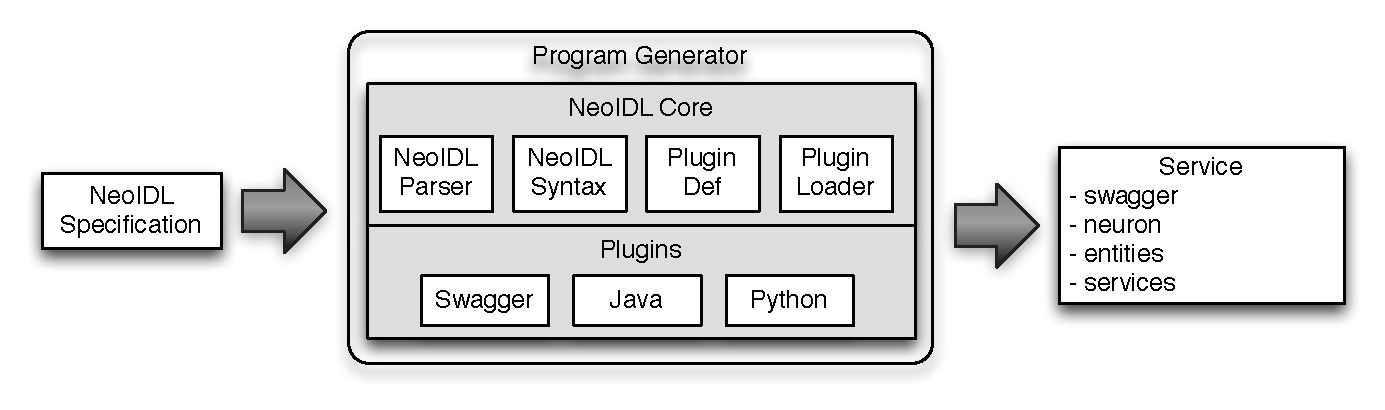
\includegraphics[scale=0.55,trim=0cm 1.5cm 0cm 0cm]{programgenerator.pdf}
\vspace{-.5cm}
\end{center}
\caption{Major architectural components of \neoidl{} program generator}
\label{fig:programGenerator}
\end{figure*}

\section{NeoIDL Design}\label{sec:design}

In this section we first present an overview of our approach (Section~\ref{sub:approachOverview}), which
consists of a specification language and a program generator. Then, in
Section~\ref{sub:langConstructs}, we detail the principal constructs of \neoidl{} and
illustrate some examples of service specifications. Sections~\ref{sub:lexical} and~\ref{sub:syntactic} present 
the lexical and syntactic structure of \neoidl. 

\subsection{Approach Overview}\label{sub:approachOverview}

NeoIDL has been developed to enable the specification of REST 
services and to allow the code generation for the implementation 
of those services for specific platforms.
It aims to simplify the development of
services, by generating code from a
service specification. Figure~\ref{fig:programGenerator} illustrates
the main components of our approach, which consists
of: (i) a domain-specific language (\neoidl)
for specifying REST services with their respective
contracts; and (ii) a
program generator that enables the code generation of REST services
in different platforms. 
The \neoidl{} generator is structured as a set of
core modules, which are responsible for the parsing,
syntax definition, and processing of \neoidl{} specifications;
as well as modules for the definition and
management of \neoidl{} plugins. Each \neoidl{} plugin
defines specific extensions for the code generator
that enables the generation of REST services for different platforms
or programming languages.

The current implementation of \neoidl{} has been already used
to enable the generation of services for the \neocortex{} platform and the open-source 
Python Twisted Framework~\cite{twisted:book}. The \neocortex{} platform is 
a proprietary framework designed by the Brazilian Army that implements 
a service-oriented architecture based on
REST. \neocortex{} has been developed using  NodeJS---a cross-platform
runtime environment for server-side and networking applications.
The main reasons for
developing \neocortex{}, instead of using existing frameworks for 
SOC, are related to specific needs to deploy services in
different platforms, ranging from well structured environments to
small devices (such as tablets and mobile phones), as well as different
networking environments (including eventually-connected half-duplex
radio channels). In addition,
\neocortex{} presents a polyglot solution that supports 
the deployment of services written in different languages (such as
Python and Java) and addresses high responsiveness requirements using
reactive and asynchronous programming techniques. 

Each \neocortex{} service must provide a contract 
and a \emph{front-controller}---which delegates a service request to the 
corresponding implementation.  
Even simple \neocortex{} services require
different components that implement business logic and other
concerns, such as concurrency and
persistence. In a nutshell, a 
typical \neocortex{} service comprises several
components as depicted in Figure~\ref{fig:message}, which shows 
the internal components of a \neocortex{} service for sending and 
receiving messages, including: 

\begin{itemize}
\item The \texttt{synapse}
component exposes the service API using a Swagger based JSON
specification, which provides an useful interface for testing a service.  

\item The \texttt{neuron} component implements the necessary behavior for initializing and
  stopping a service, as well it is responsible for mapping a requested URL pattern into
  a specific resource class. 

\item Business and utility logic that implements the expected behavior for a service 
  and user defined data types represented as domain classes. Often, 
  these components are written either in Python or Java (or any other language supported by \neocortex). 
  In the cases where it is necessary to persist a data type on a database, a database mapping is also
  necessary within a service.  
\end{itemize}





\begin{figure}[hbt]
\begin{center}
\vspace{-.5cm}
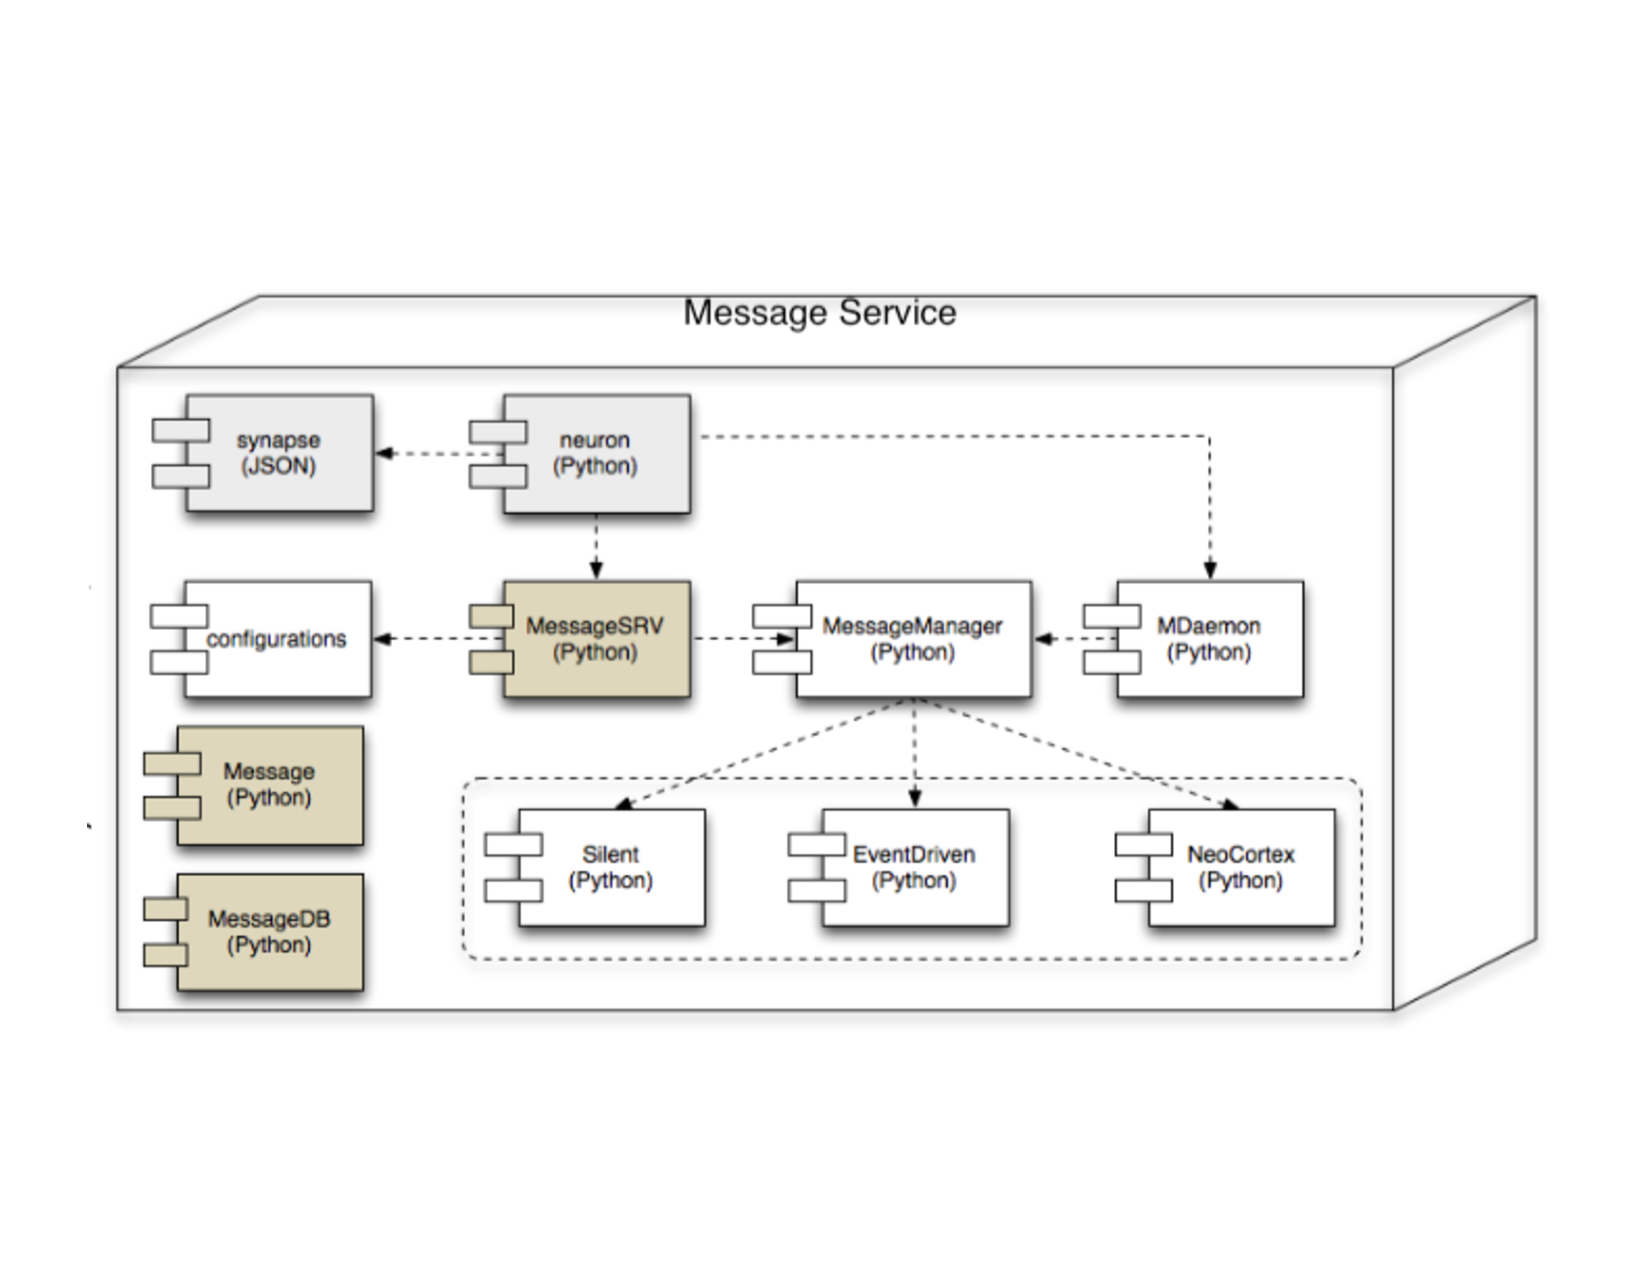
\includegraphics[scale=0.4,trim=0cm 5cm 0cm 4.5cm]{message.pdf}
\vspace{-.3cm}
\end{center}
\caption{Components related to a \neocortex{} message service.}
\label{fig:message}
\end{figure}


In the context of \neocortex{}, we translate \neoidl{} specifications into
Swagger specifications and other software components for 
different programming languages--- to fulfill the polyglot requirement
of \neocortex. 
Actually, \neoidl{} generates code for five types of components: 
\texttt{synapse}, \texttt{neuron}, resource classes
(\texttt{MessageSRV}), domain classes (\texttt{Message}), 
and database mapping (\texttt{MessageDB}).
It is important to note that only 
the first two components should not be manually customized; whereas
the remaining ones should not be overwritten by a \neoidl{}
translation---in the cases they have been manually edited. 


The polyglot requirement of \neocortex{} motivated us to implement 
the program generator of \neoidl{} as a pluggable architecture 
(see Figure~\ref{fig:programGenerator})---so that
we are able to evolve the code generation support in a modular
way. For instance, implementing a C++ program generator from \neoidl{}
specifications does not require any change in the existing code of the
program generator. It is only necessary to implement a new \neoidl{}
plugin. 









\subsection{NeoIDL Language}\label{sub:langConstructs}

\neoidl{} simplifies service specifications by means of 
(a) mechanisms for modularizing and inheriting user defined data 
types, and (b) a concise syntax that is quite similar to the 
\emph{interface description languages} of Apache Thrift or CORBA. A 
\neoidl{} specification might be split into modules, where each
module contains several definitions. In essence, a \neoidl{} definition might be either a 
data type (using the \texttt{entity} construct) or a service describing
operations that might be reached by a given pair (URI, HTTP
method). Figures~\ref{lst:messagedata-neo}
and~\ref{lst:sentmessage-neo} present two \neoidl{} modules:
(i) the data-oriented \texttt{MessageData} module;
and the service-oriented \texttt{Message} module.

The \texttt{MessageData} module (Figure~\ref{lst:messagedata-neo})
declares an enumeration
(\texttt{MessageType}), which states the two valid types of
messages (a message must be either a \emph{message sent} or
a \emph{message received}); and a data type (\texttt{Message}),
which details the expected structure of a
message. We use a \emph{convention over configuration approach}, 
assuming that all attributes of a user defined data type are
mandatory, though it is possible to specify an attribute as being optional  
using the syntax \texttt{<Type> <Ident> = 0;}, as exemplified by
the \texttt{subject} field of the \texttt{Message} data type.

\begin{figure}[htb]
\begin{small}
\lstinputlisting[language=NeoIDL,firstnumber=1]{mensagemData.tex}
\vspace{-.5cm}
\end{small}
\caption{Message data type specified in \neoidl}
\label{lst:messagedata-neo}
\end{figure}

The \texttt{Message} module of Figure~\ref{lst:sentmessage-neo}
specifies one service resource (\texttt{sentbox}). As explained,
we send requests for the methods of a given resource using a specific
path. In the example, the \texttt{sentbox} resource's
methods are available from the relative path
\texttt{/messages/sent}. This resource declares 
 two operations: one
\method{POST} method that might be used for
sending messages and one \method{GET} method 
that might be used for listing all messages
sent from a given sequential number.

Also according to our \emph{convention over configuration}
approach, we assume
that the arguments of \method{POST} and \method{PUT} operations
are sent in the 
request body, whereas arguments of \method{GET} operations are
either sent enclosed
with the request URL or enclosed with the URL path (in a similar way
as \method{DELETE} operations). We are able to change these conventions by
using specific annotations attached to an operation parameter.  In
these examples, conventions are used to reduce the size of services'
specifications. 

\begin{figure}[htb]
\begin{small}
\lstinputlisting[language=NeoIDL,firstnumber=1]{mensagem.tex}
\end{small}
\caption{Sent message service specification in \neoidl}
\label{lst:sentmessage-neo}
\end{figure}

To support language extensibility, \neoidl{}
specifications can be augmented through annotations. The main reason
for introducing annotations in \neoidl{} was the possibility to extend
the semantics of a specification without the need to change the 
concrete syntax of \neoidl. For instance, suppose that we want to 
express security policies for a service resource. A developer could 
change the concrete syntax of \neoidl{} for this purpose, defining new
language constructs for specifying the authentication method (based on
tokens or user passwords), the cryptographic algorithm used in the
resource request and response, and the role-based permissions to the
resource capabilities. However,
changing the concrete syntax to allow the specification of
unanticipated properties of a resource often breaks the code of the program
generator. 

Instead,
using annotations, developers might extend the language within \neoidl{}
specifications. Therefore, apart from the \neoidl{} definitions
discussed before, it is also possible to define new annotations that
might be attached to the fundamental constructs of \neoidl{} (i.e.
\texttt{module}, \texttt{enum}, \texttt{entity}, and
\texttt{resource}). Each annotation consists of a name, a target
element that indicates the \neoidl{} constructs the annotation 
might be attached to, and a list of properties. When transforming 
a specification, the list of annotations attached to a \neoidl{}
element is available to the plugins, which could consider the 
additional semantics during the program generation. Figure~\ref{lst:agent}
presents a \neoidl{} example that attaches an user defined
annotation (\texttt{SecurityPolicy}) to specify security policies 
on the \texttt{agent} resource. In the example, 
using the \texttt{SecurityPolicy} annotation we specify
that the operations of the \texttt{agent} resource
(i) must use a basic authentication mechanism, (ii)
the arguments and return values must be encoded using the
AES algorithm, and (iii) only authenticated users
having the \emph{admin} role are authorized to request the
resources. 

 
\begin{figure}
\begin{small}
\lstinputlisting[language=NeoIDL,firstnumber=1]{agent.tex}
\vspace{-.5cm}
\end{small}
\caption{\neoidl{} specification using annotations}
\label{lst:agent}
\end{figure}

In the next sections we present the lexical and 
syntactic structures of NeoIDL, considering 
the revision of August 23, 2015. Both sections 
were (almost) automatically generated by the BNF-Converter~\cite{forsberg-bnfc:2004} 
parser generator. 

\newcommand{\emptyP}{\mbox{$\epsilon$}}
\newcommand{\terminal}[1]{\mbox{{\texttt {#1}}}}
\newcommand{\nonterminal}[1]{\mbox{$\langle \mbox{{\sl #1 }} \! \rangle$}}
\newcommand{\arrow}{\mbox{::=}}
\newcommand{\delimit}{\mbox{$|$}}
\newcommand{\reserved}[1]{\mbox{{\texttt {#1}}}}
\newcommand{\literal}[1]{\mbox{{\texttt {#1}}}}
\newcommand{\symb}[1]{\mbox{{\texttt {#1}}}}

\subsection{The lexical structure of NeoIDL}\label{sub:lexical}

\subsubsection*{Identifiers}

Identifiers \nonterminal{Ident} are unquoted strings beginning with a letter,
followed by any combination of letters, digits, and the characters {\tt \_ '},
reserved words excluded.

\subsubsection*{Literals}

String literals \nonterminal{String}\ have the form
\terminal{``}$x$\terminal{``}, where $x$ is any sequence of any characters
except \terminal{``}\ unless preceded by \text{\tt \char92{}}.

Integer literals \nonterminal{Int}\ are nonempty sequences of digits.

Double-precision float literals \nonterminal{Double}\ have the structure
indicated by the regular expression $\nonterminal{digit}+ \mbox{{\it `.'}} 
\nonterminal{digit}+ (\mbox{{\it `e'}} \mbox{{\it `-'}}? \nonterminal{digit}+)?$ i.e.
two sequences of digits separated by a decimal point, optionally
followed by an unsigned or negative exponent.

\subsubsection*{Reserved words and symbols}
The set of reserved words is the set of terminals appearing in the grammar. 
Those reserved words that consist of non-letter characters are called symbols, 
and they are treated in a different way from those that are similar to identifiers. 
The lexer follows rules familiar from languages like Haskell, C, and Java, including longest match and spacing conventions.

The reserved words used in NeoIDL are the following: \\

\begin{tabular}{lll}
{\reserved{annotation}} &{\reserved{call}} &{\reserved{entity}} \\
{\reserved{enum}} &{\reserved{extends}} &{\reserved{float}} \\
{\reserved{for}} &{\reserved{import}} &{\reserved{int}} \\
{\reserved{module}} &{\reserved{path}} &{\reserved{resource}} \\
{\reserved{string}} & & \\
\end{tabular}\\
  
The symbols used in NeoIDL are the following: \\

\begin{tabular}{lll}
{\symb{\{}} &{\symb{\}}} &{\symb{;}} \\
{\symb{{$=$}}} &{\symb{.}} &{\symb{@}} \\
{\symb{(}} &{\symb{)}} &{\symb{0}} \\
{\symb{{$=$}{$=$}}} &{\symb{{$<$}{$>$}}} &{\symb{{$>$}}} \\
{\symb{{$>$}{$=$}}} &{\symb{{$<$}}} &{\symb{{$<$}{$=$}}} \\
{\symb{[}} &{\symb{]}} &{\symb{@get}} \\
{\symb{@post}} &{\symb{@put}} &{\symb{@delete}} \\
{\symb{/@require}} &{\symb{/@ensure}} &{\symb{/@invariant}} \\
{\symb{/@otherwise}} &{\symb{/**}} &{\symb{*/}} \\
{\symb{*}} &{\symb{@desc}} &{\symb{@param}} \\
{\symb{@consume}} &{\symb{,}} & \\
\end{tabular}\\

\subsection{The syntactic structure of NeoIDL}\label{sub:syntactic}

Non-terminals are enclosed between $\langle$ and $\rangle$. 
The symbols  {\arrow}  (production),  {\delimit}  (union) 
and {\emptyP} (empty rule) belong to the following BNF notation.
All other symbols are terminals.\\

\begin{small}
\begin{tabular}{lll}
\label{lst:BNFnot}
{\nonterminal{Modulo}} {\arrow} {\terminal{module}} {\nonterminal{Ident}} {\terminal{\{}} \\ 
 \quad {\nonterminal{ListImport}} \\ 
 \quad {\nonterminal{MPath}} \\ 
 \quad {\nonterminal{ListEnum}} \\ 
 \quad {\nonterminal{ListEntity}} \\ 
 \quad {\nonterminal{ListResource}} \\ 
 \quad {\nonterminal{ListDecAnnotation}} \\ 
{\terminal{\}}}  \\
\end{tabular}\\

\begin{tabular}{lll}
{\nonterminal{Import}} & {\arrow}  &{\terminal{import}} {\nonterminal{NImport}} {\terminal{;}}  \\
\end{tabular}\\

\begin{tabular}{lll}
{\nonterminal{MPath}} & {\arrow}  &{\emptyP} \\
 & {\delimit}  &{\terminal{path}} {\terminal{{$=$}}} {\nonterminal{String}} {\terminal{;}}  \\
\end{tabular}\\

\begin{tabular}{lll}
{\nonterminal{NImport}} & {\arrow}  &{\nonterminal{Ident}}  \\
 & {\delimit}  &{\nonterminal{Ident}} {\terminal{.}} {\nonterminal{NImport}}  \\
\end{tabular}\\

\begin{tabular}{lll}
{\nonterminal{Entity}} & {\arrow}  &{\nonterminal{ListDefAnnotation}} {\terminal{entity}} {\nonterminal{Ident}} {\terminal{\{}} {\nonterminal{ListProperty}} {\terminal{\}}} {\terminal{;}}  \\
 & {\delimit}  &{\nonterminal{ListDefAnnotation}} {\terminal{entity}} {\nonterminal{Ident}} {\terminal{extends}} {\nonterminal{Ident}} {\terminal{\{}} {\nonterminal{ListProperty}} {\terminal{\}}} {\terminal{;}}  \\
\end{tabular}\\

\begin{tabular}{lll}
{\nonterminal{Enum}} & {\arrow}  &{\terminal{enum}} {\nonterminal{Ident}} {\terminal{\{}} {\nonterminal{ListValue}} {\terminal{\}}} {\terminal{;}}  \\
\end{tabular}\\

\begin{tabular}{lll}
{\nonterminal{DecAnnotation}} & {\arrow}  &{\terminal{annotation}} {\nonterminal{Ident}} {\terminal{for}} {\nonterminal{AnnotationType}} {\terminal{\{}} {\nonterminal{ListProperty}} {\terminal{\}}} {\terminal{;}}  \\
\end{tabular}\\

\begin{tabular}{lll}
{\nonterminal{DefAnnotation}} & {\arrow}  &{\terminal{@}} {\nonterminal{Ident}} {\terminal{(}} {\nonterminal{ListAssignment}} {\terminal{)}} {\terminal{;}}  \\
\end{tabular}\\

\begin{tabular}{lll}
{\nonterminal{Parameter}} & {\arrow}  &{\nonterminal{Type}} {\nonterminal{Ident}} {\nonterminal{Modifier}}  \\
\end{tabular}\\

\begin{tabular}{lll}
{\nonterminal{Assignment}} & {\arrow}  &{\nonterminal{Ident}} {\terminal{{$=$}}} {\nonterminal{Value}}  \\
\end{tabular}\\

\begin{tabular}{lll}
{\nonterminal{Modifier}} & {\arrow}  &{\emptyP} \\
 & {\delimit}  &{\terminal{{$=$}}} {\terminal{0}}  \\
\end{tabular}\\

\begin{tabular}{lllllllll}
{\nonterminal{AnnotationType}} & {\arrow}  &{\terminal{resource}}  
 & {\delimit}  &{\terminal{enum}}  
 & {\delimit}  &{\terminal{entity}}  
 & {\delimit}  &{\terminal{module}} 
\end{tabular}\\

\begin{tabular}{lll}
{\nonterminal{Resource}} & {\arrow}  &{\nonterminal{ListDefAnnotation}} {\terminal{resource}} {\nonterminal{Ident}} {\terminal{\{}} {\terminal{path}} {\terminal{{$=$}}} {\nonterminal{String}} {\terminal{;}} {\nonterminal{ListCapacity}} {\terminal{\}}} {\terminal{;}}  \\
\end{tabular}\\

\begin{tabular}{lll}
{\nonterminal{Capacity}} & {\arrow}  &{\nonterminal{NeoDoc}} {\nonterminal{ListDefNAnnotation}} {\nonterminal{Method}} {\nonterminal{Type}} {\nonterminal{Ident}} {\terminal{(}} {\nonterminal{ListParameter}} {\terminal{)}} {\terminal{;}}  \\
\end{tabular}\\


\begin{tabular}{lllllllll}
{\nonterminal{Method}} & {\arrow}  &{\terminal{@get}} 
 & {\delimit}  &{\terminal{@post}} 
 & {\delimit}  &{\terminal{@put}}  
 & {\delimit}  &{\terminal{@delete}} 
\end{tabular}\\
\end{small}    



\subsection{Summary of Our Approach}

We end this section by highlighting that
the design of \neoidl{} comprises a domain specific
language (DSL) for specifying services APIs in a REST based environment and 
an extensible program generator that might evolve to generate code to
different platforms and programming languages.
Next section presents some details
about the \neoidl{} implementation,
which uses Haskell as programming language--- a well known language 
for building (embedded) DSLs~\cite{hudak-dsl1}. 
 

  
\section{NeoIDL Implementation}\label{sec:implementation}

As shown in Figure~\ref{fig:programGenerator}, the implementation of \neoidl{} consists of a core (split into
several Haskell modules) and 
several plugins, one for each target language (such as Swagger,
Python, or Java). The core module includes a tiny application that loads 
plugins definition and processes the program arguments, which 
specify the input \neoidl{} file, the output directory, and the languages that should be generated code from the 
input file. Moreover, the core module contains a
parser and a type checker for \neoidl{} specifications. 
We have developed the parser for \neoidl{} using \bnfc~\cite{ranta-bnfc:2012}, 
an easy to use parser generator that takes as
input a syntax specification and generates code (both abstract syntax and
parser) for different languages, including Haskell. Figure~\ref{fig:neoidl-architecture}
represents an architectural abstraction of \neoidl{} program
generator. 

\begin{figure}[b]
\begin{center}
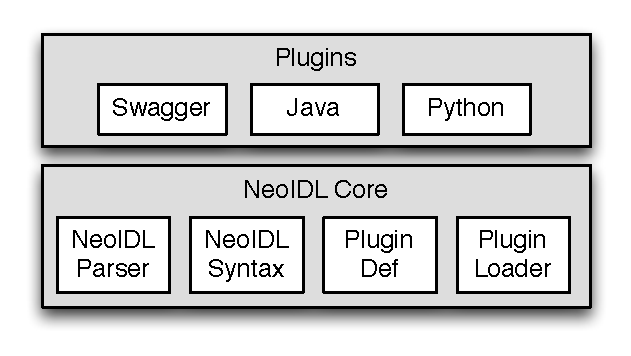
\includegraphics[scale=0.6]{neoidl.pdf}
\vspace{-.5cm}
\end{center}
\caption{Major architectural components of \neoidl{} program generator.}
\label{fig:neoidl-architecture} 
\end{figure}

In the remaining of this section
we present details about the implementation of two
\neoidl{} Haskell modules: 
\texttt{PluginDef} and \texttt{PluginLoader}. The first states the
organization of a \neoidl{} plugin and the second is responsible for
loading all available plugins. The details here are
particularly useful for those who want to develop extensible architectures
using Haskell. 


\subsection{PluginDef component}{\label{sec:plugindef}}

\neoidl{} plugins must comply 
with a few design rules that \texttt{PluginDef}
states. \texttt{PluginDef} is a Haskell module that 
declares two data types (\texttt{Plugin} and
\texttt{GeneratedFile}) and a type signature
(\texttt{Transform = Module -> [GeneratedFile]}) 
defining a family of functions that map a \neoidl{} module into 
a list of files whose contents are the results of the 
transformation process.

According to these design rules, each \neoidl{} plugin must declare an instance of the
\texttt{Plugin} data type and implement functions according to the
\texttt{Transform} type signature. Moreover, the 
\texttt{Plugin} instance must be named as \texttt{plugin}, so that the
\texttt{PluginLoader} component will be able to obtain the necessary 
data for executing a given plugin. Indeed, the execution of a plugin
consists of applying the respective \texttt{transformation} function for a
\neoidl{} module, producing as result a list of files that consists of 
a name and a \texttt{Doc} as file content.\footnote{The \texttt{Doc} data type
comes from the John Hughes Pretty Printer library.}  

As an alternative, we could have implemented a Haskell type class~\cite{jones-typeClasses:1995} 
exposing operations for obtaining the necessary data for a given
plugin. Although this approach might seem more natural for specifying
design rules for a pluggable architecture in Haskell, in the end it
would lead to a cumbersome approach to our problem. The main reason
for discarding this alternative approach was the need to (a) implement 
a data type, (b) make this data type an instance of the mentioned type
class, and (c) create an instance of that data type. All those steps
would be necessary for each plugin. Using our approach, the obligation
of a plugin developer is just to provide an instance of the
\texttt{Plugin} datatype, taking into account the name convention we
mentioned above. 
The \texttt{language} attribute of the \texttt{Plugin} datatype
is used for UI purpose only, so that the users will be able to obtain the list of available
plugins and select which plugins will be used during a program generation.  

\begin{figure}[htb]
\begin{hscode}\SaveRestoreHook
\column{B}{@{}>{\hspre}l<{\hspost}@{}}\column{3}{@{}>{\hspre}l<{\hspost}@{}}\column{9}{@{}>{\hspre}l<{\hspost}@{}}\column{16}{@{}>{\hspre}l<{\hspost}@{}}\column{E}{@{}>{\hspre}l<{\hspost}@{}}\>[B]{}\mathbf{module}\;\Conid{PluginDef}\;\mathbf{where}{}\<[E]\\[\blanklineskip]\>[B]{}\mathbf{data}\;\Conid{Plugin}\mathrel{=}\Conid{Plugin}\;\{\mskip1.5mu {}\<[E]\\
\>[B]{}\hsindent{3}{}\<[3]\>[3]{}\Varid{language}{}\<[16]\>[16]{}\mathbin{::}\Conid{String},{}\<[E]\\
\>[B]{}\hsindent{3}{}\<[3]\>[3]{}\Varid{transformation}\mathbin{::}\Conid{Transformation}{}\<[E]\\
\>[B]{}\mskip1.5mu\}{}\<[E]\\[\blanklineskip]\>[B]{}\mathbf{data}\;\Conid{GeneratedFile}\mathrel{=}\Conid{GeneratedFile}\;\{\mskip1.5mu {}\<[E]\\
\>[B]{}\hsindent{3}{}\<[3]\>[3]{}\Varid{name}{}\<[9]\>[9]{}\mathbin{::}\Conid{String},{}\<[E]\\
\>[B]{}\hsindent{3}{}\<[3]\>[3]{}\Varid{content}\mathbin{::}\Conid{Doc}{}\<[E]\\
\>[B]{}\mskip1.5mu\}{}\<[E]\\[\blanklineskip]\>[B]{}\mathbf{type}\;\Conid{Transformation}\mathrel{=}\Conid{Module}\to [\mskip1.5mu \Conid{GeneratedFile}\mskip1.5mu]{}\<[E]\ColumnHook
\end{hscode}\resethooks
\caption{\texttt{PluginDef} component.}
\label{fig:plugindef}
\end{figure}

\subsection{PluginLoader component}

Based on the design rules discussed in the previous section, 
the \texttt{PluginLoader} component is able to dynamically 
load the available \neoidl{} plugins. This is a Haskell
module (see Figure~\ref{lst:loader}) that exposes the
\texttt{loadPlugins} function, which returns a list  with all
available plugins. This list is obtained by compiling the Haskell plugin modules 
during the program execution and dynamically evaluating an 
expression that yields a list of \texttt{Plugin} datatype instances. 

\begin{figure}[htb]
\begin{hscode}\SaveRestoreHook
\column{B}{@{}>{\hspre}l<{\hspost}@{}}\column{3}{@{}>{\hspre}l<{\hspost}@{}}\column{4}{@{}>{\hspre}l<{\hspost}@{}}\column{5}{@{}>{\hspre}l<{\hspost}@{}}\column{6}{@{}>{\hspre}l<{\hspost}@{}}\column{7}{@{}>{\hspre}l<{\hspost}@{}}\column{8}{@{}>{\hspre}l<{\hspost}@{}}\column{16}{@{}>{\hspre}l<{\hspost}@{}}\column{26}{@{}>{\hspre}l<{\hspost}@{}}\column{E}{@{}>{\hspre}l<{\hspost}@{}}\>[B]{}\mathbf{module}\;\Conid{PluginLoader}\;(\Varid{loadPlugins})\;\mathbf{where}{}\<[E]\\[\blanklineskip]\>[B]{}\mathbf{type}\;\Conid{HSFile}\mathrel{=}\Conid{String}{}\<[E]\\[\blanklineskip]\>[B]{}\Varid{dir}\mathbin{::}\Conid{String}{}\<[E]\\
\>[B]{}\Varid{dir}\mathrel{=}\text{\tt \char34 Plugins\char34}{}\<[E]\\[\blanklineskip]\>[B]{}\Varid{loadPlugins}\mathbin{::}\Conid{IO}\;[\mskip1.5mu \Conid{Plugin}\mskip1.5mu]{}\<[E]\\
\>[B]{}\Varid{loadPlugins}\mathrel{=}{}\<[E]\\
\>[B]{}\hsindent{3}{}\<[3]\>[3]{}\mathbf{let}{}\<[E]\\
\>[3]{}\hsindent{1}{}\<[4]\>[4]{}\Varid{pattern}\mathrel{=}\Varid{isSuffixOf}\;{}\<[26]\>[26]{}\text{\tt \char34 hs\char34}{}\<[E]\\
\>[3]{}\hsindent{1}{}\<[4]\>[4]{}\Varid{path}\;\Varid{file}\mathrel{=}\Varid{dir}\mathbin{</>}\Varid{file}{}\<[E]\\
\>[B]{}\hsindent{3}{}\<[3]\>[3]{}\mathbf{in}\;(\Varid{list}\;\Varid{dir})\bind (\Varid{compile}\mathbin{\circ}\Varid{map}\;\Varid{path}\mathbin{\circ}\Varid{filter}\;\Varid{pattern}){}\<[E]\\[\blanklineskip]\>[B]{}\Varid{dfm}\mathrel{=}\Varid{defaultFatalMessager}{}\<[E]\\
\>[B]{}\Varid{flushOut}\mathrel{=}\Varid{defaultFlushOut}{}\<[E]\\[\blanklineskip]\>[B]{}\Varid{compile}\mathbin{::}[\mskip1.5mu \Conid{HSFile}\mskip1.5mu]\to \Conid{IO}\;[\mskip1.5mu \Conid{Plugin}\mskip1.5mu]{}\<[E]\\
\>[B]{}\Varid{compile}\;\Varid{modules}\mathrel{=}{}\<[E]\\
\>[B]{}\hsindent{3}{}\<[3]\>[3]{}\Varid{defaultErrorHandler}\;\Varid{dfm}\;\Varid{flushOut}\mathbin{\$}\mathbf{do}{}\<[E]\\
\>[3]{}\hsindent{3}{}\<[6]\>[6]{}\Varid{result}\leftarrow \Varid{runGhc}\;(\Conid{Just}\;\Varid{libdir})\mathbin{\$}\mathbf{do}{}\<[E]\\
\>[6]{}\hsindent{2}{}\<[8]\>[8]{}\mathbf{let}\;\Varid{hsModules}\mathrel{=}\Varid{map}\;\Varid{haskellModule}\;\Varid{modules}{}\<[E]\\
\>[6]{}\hsindent{2}{}\<[8]\>[8]{}\mbox{\onelinecomment  five lines of (boilerplate) code are necessary to }{}\<[E]\\
\>[6]{}\hsindent{2}{}\<[8]\>[8]{}\mbox{\onelinecomment  dynamically compile Haskell code using GHC}{}\<[E]\\
\>[6]{}\hsindent{1}{}\<[7]\>[7]{}\mathbf{let}\;\Varid{exp}\mathrel{=}\Varid{buildExpresson}\;\Varid{hsModules}{}\<[E]\\
\>[6]{}\hsindent{1}{}\<[7]\>[7]{}\Varid{plugins}\leftarrow \Varid{compileExpr}\;(\Varid{exp}\plus \text{\tt \char34 ::[Plugin]\char34}){}\<[E]\\
\>[6]{}\hsindent{1}{}\<[7]\>[7]{}\Varid{return}\;\Varid{unsafeCoerce}\;\Varid{plugins}\mathbin{::}[\mskip1.5mu \Conid{Plugin}\mskip1.5mu]{}\<[E]\\
\>[3]{}\hsindent{3}{}\<[6]\>[6]{}\Varid{return}\;\Varid{result}{}\<[E]\\[\blanklineskip]\>[B]{}\Varid{buildExpression}\mathbin{::}[\mskip1.5mu \Conid{HSModule}\mskip1.5mu]\to \Conid{String}{}\<[E]\\
\>[B]{}\Varid{buildExpression}\;\Varid{hsms}\mathrel{=}\text{\tt \char34 [\char34}\plus \Varid{plugins}\plus \text{\tt \char34 ]\char34}{}\<[E]\\
\>[B]{}\hsindent{3}{}\<[3]\>[3]{}\mathbf{where}{}\<[E]\\
\>[3]{}\hsindent{2}{}\<[5]\>[5]{}\Varid{plugins}\mathrel{=}{}\<[16]\>[16]{}\Varid{concatMap}\;(\lambda \Varid{x}\to \Varid{x}\plus \text{\tt \char34 .plugin\char34})\;\Varid{hsms}{}\<[E]\\
\>[3]{}\hsindent{2}{}\<[5]\>[5]{}\Varid{concat}\mathrel{=}\Varid{join}\;\text{\tt \char34 ,\char34}{}\<[E]\ColumnHook
\end{hscode}\resethooks
\caption{\texttt{PluginLoader} component.}
\label{lst:loader}
\end{figure}

We assume that
all Haskell modules within the top level \texttt{Plugins} directory must have a plugin
definition, according to the design rules of Section~\ref{sec:plugindef}.  
In Figure~\ref{lst:loader}, the \texttt{loadPlugins} function lists all files within the
\texttt{Plugins} directory, filters the Haskell files (files
 with the \texttt{``.hs''} extension), creates a qualified name to these
 files, and applies the \texttt{compile} function to the resulting
 list of qualified names. In the next step, the \texttt{compile}
 function uses the GHC API~\cite{ghc-api}
 for compiling the Haskell modules with plugin definitions and to
 evaluate an expression that produces a list with the available
 plugins. 

Our dynamic approach for loading plugins relies on the 
 GHC API, using a specific idiom to compile Haskell
 modules and execute expressions. Figure~\ref{lst:loader} shows that
 idiom in the definition of the \texttt{compile} function, although we omit some boilerplate code that is 
 necessary to compile Haskell modules using the GHC API. The last four lines of \texttt{compile} are specific to the program generator of \neoidl.
First, we build a string representation of a Haskell \texttt{list} comprising 
 all instances of the \texttt{Plugin} datatype, obtained from the
 different \neoidl{} plugins. Then, we evaluate this string
 representation of a plugin list using the \emph{meta-programming} ability
 of the \texttt{compileExpr} function, which is available in the GHC
 API. Thus, \texttt{compileExpr} dynamically evaluates a string representation of an
 expression, which leads to a value that could be used by other
 functions of a program. 
The call to \texttt{compileExpr}  
also checks the design rule that requires 
(a) a \texttt{plugin} definition
within all \neoidl{} plugins; and (b) that  
definition must be an instance of the \texttt{Plugin} data type. 
In the cases where a plugin (exposed as a Haskell module on the
top-level Plugins directory) does not comply with this design rule, 
a runtime error occurs. Accordingly, we use the default error 
handler of GHC API to report problems when loading a plugin. 
This is a new approach of using the GHC
API to dynamically check Haskell modules in pluggable architectures. 


As an example of design rule violation in the \neoidl{} architecture, 
if there is no \texttt{plugin} definition within a
plugin, the following error is reported at runtime:

\begin{tabbing}\tt
~\char36{}\char46{}\char47{}neoIDL\\
\tt ~neoIDL\char58{}~panic\char33{}~\char40{}the~\char39{}impossible\char39{}~happened\char41{}\\
\tt ~~\char40{}GHC~version~7\char46{}6\char46{}3~for~x86\char95{}64\char45{}darwin\char41{}\char58{}\\
\tt ~~~~Not~in~scope\char58{}~\char96{}Plugins\char46{}Python\char46{}plugin\char39{}
\end{tabbing}

In the last line of the above interactive section, 
\neoidl{} program generator reports that \texttt{plugin} is not defined within 
the Python plugin module. In a similar way, if the \texttt{plugin}
definition is available but it is not an instance of the \texttt{Plugin}
data type, a type error occurs during the execution of the \neoidl{}
program (see the reported message bellow, using a \texttt{plugin} definition
assigned to a String value). 


\begin{tabbing}\tt
~\char36{}\char46{}\char47{}neoIDL\\
\tt ~neoIDL\char58{}~panic\char33{}~\char40{}the~\char39{}impossible\char39{}~happened\char41{}\\
\tt ~\char40{}GHC~version~7\char46{}6\char46{}3~for~x86\char95{}64\char45{}darwin\char41{}\char58{}\\
\tt ~~Couldn\char39{}t~match~expected~type~\char96{}Plugin\char39{}\\
\tt ~~~with~actual~type~\char96{}\char91{}GHC\char46{}Types\char46{}Char\char93{}\char39{}
\end{tabbing}

Therefore, we are using GHC API to type check Haskell modules (note that Haskell is a statically typed language) during
the loading phase of a \neoidl{} execution. Next section presents the assessment of \neoidl{} considering different 
goals. 


  

\section{Evaluation}\label{sec:assessment}

In this section we describe an evaluation of the
\neoidl{} approach through the development and generation 
of services in the context of a Brazilian
Army projects.
We first present our experience using 
\neoidl{} in that domain (Section~\ref{sub:experience}). Then, in
Section~\ref{sub:roi} we present a discussion about the 
return on investment (ROI) related to the design and development of
\neoidl. In Section~\ref{sub:modularity} we present a
technical evaluation about the modular design of \neoidl{}. Finally, in Section~\ref{sub:neoIDLandSwagger}, 
we investigate the expressiveness of \neoidl{} by comparing the size 
of existing Swagger specifications and the size of equivalent specifications 
in \neoidl.  This evaluation aims at (a) understanding the \neoidl{} benefits under the ROI 
perspective, (b) reasoning about the modular mechanisms of \neoidl{}
design, and (c) investigating the syntactic structure of \neoidl. 

Therefore, in the remaining of this section we answer the following questions:

\begin{itemize}
 \item when the design of \neoidl{} pays off?
 \item is the \neoidl{} design extensible? 
 \item what is the expressiveness of \neoidl?
\end{itemize}

We use \emph{source lines of code} as the metric to answer the first
and third questions. We investigate the second question by means of a 
qualitative assessment that considers the effort to understand, test,
and implement \neoidl{} plugins.
 
\subsection{The use of \neoidl{} in a real context}\label{sub:experience}

We have developed nine services that implement operations related to 
the domain of Command and Control (C2)~\cite{david:commandControl}. 
These services comprehend almost 50 resources and 
3000 lines of Python code. Therefore, all these services have been
implemented in Python, though other projects have been implemented in
Java as well. Here we concentrate our analysis to the services implemented
in Python. 

Approximately, the number of lines of Python code related to 
our service repository increases according to the 
function $sloc = 330 \times numberOfServices$--- since, in average, each
service requires about 330 lines of Python code (with a standard
deviation of 119). It is important to note that services are often
implemented as a thin layer on top of existing components that
implement reusable tasks or business logic. Accordingly, to understand
the impact of \neoidl{} accurately, here we do not consider lines of code related to (a) existing tasks and 
business logic implementations and (b) libraries that might be 
reused through different services. 
The boxplot of Figure~\ref{fig:sloc-boxplot}
summarizes the SLOC distribution among the services 
implementations. 

\begin{figure}[thb]
\begin{center}
\vspace{-1cm}
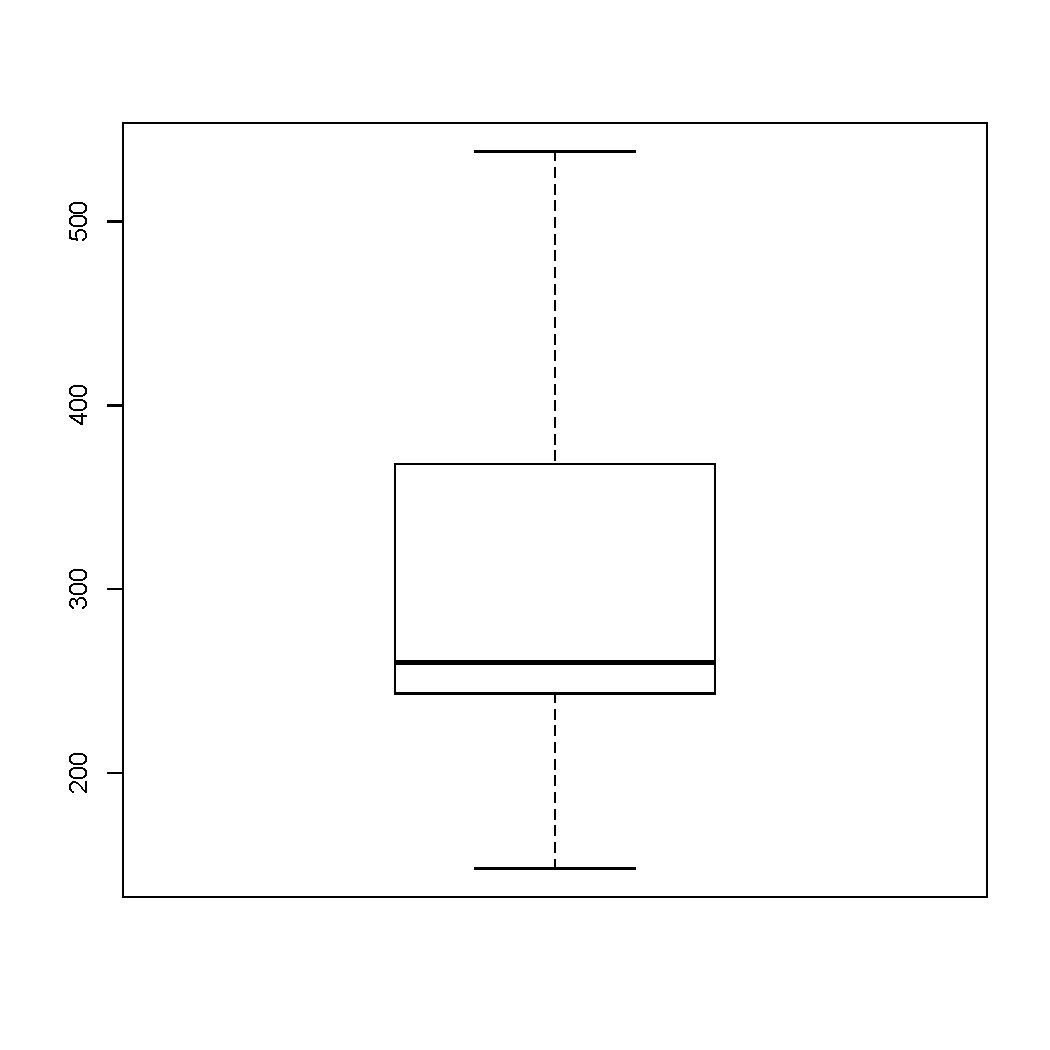
\includegraphics[scale=0.5]{sloc-boxplot.pdf}
\vspace{-1.5cm}
\end{center}
\caption{SLOC distribution among services implementations}
\label{fig:sloc-boxplot}
\end{figure}

Based on the development of these services, we estimate that 
it is possible to generate about 30\% to 50\% of
a service code using \neoidl. Indeed, in the cases that a service is
\emph{data-oriented}, involving basic operations for creating,
updating, querying and deleting data, we achieve a higher degree of
code generation. Differently, in the cases that a service encapsulates low level
behavior (such as the implementation of a \emph{chat-based} message protocol), 
we achieve a low degree of code generation using \neoidl, 
mainly because the current version of \neoidl{} does
not provide any behavioral construct. 

\subsection{Return on Investment of \neoidl}\label{sub:roi}

It is important to reason about the instant in which the design and 
development of a DSL pays off, since the related effort could not justify 
the benefits. Accordingly, here we discuss about this issue relating 
effort to \emph{source lines of code} (SLOC)~\cite{park-sloc:1992}.

\neoidl{} comprises almost 2500 lines of code,
considering the AST code generated
by \bnfc. 
Figure~\ref{graph:sloc} presents more details about the distribution
of \neoidl{} SLOC. 
Note that nearly 67\% of the Haskell code results from the
\bnfc{} parser generator. Therefore, excluding the generated code from
our analysis, as well as unit testing code and make files, \neoidl{} consists
of 740 lines of Haskell code and 50 lines of code that (a) specifies the
concrete syntax of \neoidl{} and (b) serves as input to the
\bnfc. According to the COCOMO model~\cite{bohem:2000}, it is possible to 
compute effort from SLOC using equations (1) and (2). This leads to an
effort estimation of 3.17 months, which is quite close to the real
effort to implement \neoidl{}, even considering that a significant effort on the
design of \neoidl{}  was related to the successive refinements on the concrete syntax
of the language---these refinements are not well captured within the 50
lines of code necessary to specify the concrete syntax using \bnfc.

\begin{small}
\begin{eqnarray}
personMonths & = & 2.4 \times KSLOC ^ {1.05} \\  
        & = & 2.4 \times 0.79 ^ {1.05}  \nonumber \\ 
        & = & 1.87 \nonumber \\
months & = & 2.5 \times personMonths^{0.38} \\
    & = & 2.5 \times 1.87^{0.38} \nonumber \\
    & = & 3.17 \nonumber
\end{eqnarray} 
\end{small}


\begin{figure*}[bth]
\begin{center}
\vspace{-1cm}
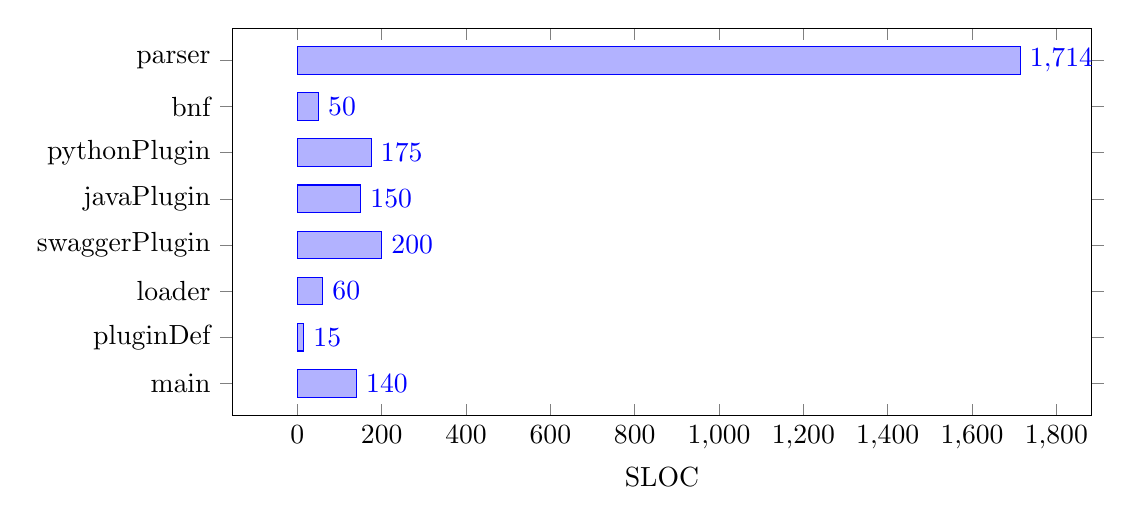
\begin{tikzpicture}
\begin{axis}[xbar, width=12.5cm, height=6.5cm, enlarge y limits=0.1,
  xlabel={SLOC}, 
  symbolic y coords={main,pluginDef,
loader,swaggerPlugin,javaPlugin,pythonPlugin,bnf,parser}, ytick=data, nodes near
  coords, nodes near coords align={horizontal}]
  \addplot coordinates {(140,main) (15,pluginDef) (60,loader)
  (200,swaggerPlugin) (150,javaPlugin) (175,pythonPlugin)(50,bnf)(1714,parser)};
\end{axis}
\end{tikzpicture}
\vspace{-.5cm}
\end{center}
\caption{\neoidl{} distribution of lines of code}
\label{graph:sloc}
\end{figure*}

For generating the Python services to the C2 domain,
the following \neoidl{} modules are necessary:
\texttt{bnf}, \texttt{loader}, \texttt{pluginDef}, \texttt{main}, 
\texttt{swaggerPlugin}, and \texttt{pythonPlugin}. These modules
totalize 640 of Haskell and BNF code.
Considering the discussion present in the previous section, 
we estimate the break-even of \neoidl{}
according to equations (3), (4), and (5). The third equation
computes the lines of code necessary for $n$ services without 
using \neoidl; whereas the fourth and fifth equations compute 
the lines of code for $n$ services, considering that \neoidl{} 
generates 30\% and 50\% of the code, respectively.  Therefore, the
break-even of \neoidl{} must be achieved after developing a number 
of services between 4 and 7 (see Figure~\ref{fig:roi}). As a consequence, we believe that 
the design and development of \neoidl{} improve software 
quality and productivity--- by reducing the need to 
write boilerplate code, at no significant additional costs.

\begin{small}
\begin{eqnarray}
sloc & = & 330 \times numberOfServices \\
sloc & = & 0.7 \times 330 \times numberOfServices + 640 \\
sloc & = & 0.5 \times 330 \times numberOfServices + 640 
\end{eqnarray}
\end{small}

\begin{figure}[thb]
\begin{center}
\vspace{-1cm}
\begin{tikzpicture}
\pgfplotsset{every axis legend/.append style={
   at={(0.5,1.03)},
   anchor=south}}
\begin{axis}[xlabel={$Number\ of\ services$}, ylabel={$SLOC$}, legend columns=3]
\addplot[smooth,mark=,black, solid] table {data2.tex}; \addlegendentry{Eq (3)}
\addplot[smooth,mark=,gray, dashed] table {data1.tex};\addlegendentry{Eq (4)}
\addplot[smooth,mark=,red,dashed] table {data3.tex};\addlegendentry{Eq (5)}
\end{axis}
\end{tikzpicture}
\end{center}
\caption{Return on investment of \neoidl}
\label{fig:roi}
\end{figure}

\vspace{-1cm}
\subsection{Modularity analysis}\label{sub:modularity}

\neoidl{} includes facilities to develop plugins and to evolve \neoidl{} specifications 
through annotations. As explained in Section~\ref{sec:implementation} we expose plugins
according to some design rules, which allow us to develop and test plugins with a
slight dependency on the existing code of the program generator. 
This encourages contributions to \neoidl, by enabling 
developers to design and implement new
plugins. In addition, it is possible to unit test a \neoidl{} plugin in
an isolated manner. Here we relate modularity to extensibility (it is
easy to contribute to \neoidl{} without a deep knowledge of 
the core components of \neoidl) and testability (it is possible to
test each \neoidl{} plugin in isolation).

Actually, to develop a plugin, it is only necessary to understand the design
rules discussed in Section~\ref{sec:implementation} 
and an external library (the John Hughes and Simon Peyton Jones Pretty
Printer library). For instance, Figure~\ref{lst:plugin} shows the 
full implementation of a \neoidl{} plugin, which reports
basic metrics of size from a \neoidl{} specification. To keep things 
simple, that plugin generates a file (named \texttt{metrics.data})
whose content 
consists of the name of a \neoidl{} module followed by three lines 
stating the number of enums, entities, and resources within that
module. Thus, the \texttt{Metrics} plugin comprises only pure Haskell 
functions, which are independent of the technologies used 
to load plugins and are quite easy to test. 

\begin{figure}[htb]
\begin{hscode}\SaveRestoreHook
\column{B}{@{}>{\hspre}l<{\hspost}@{}}\column{3}{@{}>{\hspre}l<{\hspost}@{}}\column{5}{@{}>{\hspre}l<{\hspost}@{}}\column{13}{@{}>{\hspre}l<{\hspost}@{}}\column{31}{@{}>{\hspre}l<{\hspost}@{}}\column{E}{@{}>{\hspre}l<{\hspost}@{}}\>[B]{}\mathbf{module}\;\Conid{\Conid{Plugins}.Metrics}\;(\Varid{plugin})\;\mathbf{where}{}\<[E]\\[\blanklineskip]\>[B]{}\mathbf{import}\;\Conid{\Conid{NeoIDL}.\Conid{Lang}.AbsNeoIDL}{}\<[E]\\
\>[B]{}\mathbf{import}\;\Conid{PluginDef}{}\<[E]\\[\blanklineskip]\>[B]{}\mathbf{import}\;\Conid{\Conid{Text}.\Conid{PrettyPrint}.HughesPJ}{}\<[E]\\[\blanklineskip]\>[B]{}\Varid{plugin}\mathbin{::}\Conid{Plugin}{}\<[E]\\
\>[B]{}\Varid{plugin}\mathrel{=}\Conid{Plugin}\;\{\mskip1.5mu {}\<[E]\\
\>[B]{}\hsindent{3}{}\<[3]\>[3]{}\Varid{language}\mathrel{=}\text{\tt \char34 Metrics\char34},{}\<[E]\\
\>[B]{}\hsindent{3}{}\<[3]\>[3]{}\Varid{transformation}\mathrel{=}\Varid{generateMetrics}{}\<[E]\\
\>[B]{}\mskip1.5mu\}{}\<[E]\\[\blanklineskip]\>[B]{}\Varid{print}\mathbin{::}\Conid{String}\to [\mskip1.5mu \Varid{a}\mskip1.5mu]\to \Conid{Doc}{}\<[E]\\
\>[B]{}\Varid{print}\;\Varid{str}\;\Varid{lst}\mathrel{=}\Varid{text}\;\Varid{str}\mathbin{<+>}(\Varid{text}\mathbin{\circ}\Varid{show}\mathbin{\circ}\Varid{length})\;\Varid{lst}{}\<[E]\\[\blanklineskip]\>[B]{}\Varid{generateMetrics}\mathbin{::}\Conid{Transformation}{}\<[E]\\
\>[B]{}\Varid{generateMetrics}\mathrel{=}\lambda (\Conid{Module}\;(\Conid{Ident}\;\Varid{s})\;\anonymous \;\anonymous \;\Varid{ens}\;\Varid{ess}\;\Varid{rss})\to {}\<[E]\\
\>[B]{}\hsindent{3}{}\<[3]\>[3]{}\mathbf{let}{}\<[E]\\
\>[3]{}\hsindent{2}{}\<[5]\>[5]{}\Varid{outputFile}\mathrel{=}\Conid{GeneratedFile}\;\Varid{name}\;\Varid{content}{}\<[E]\\
\>[3]{}\hsindent{2}{}\<[5]\>[5]{}\Varid{name}{}\<[13]\>[13]{}\mathrel{=}\text{\tt \char34 metrics.data\char34}{}\<[E]\\
\>[3]{}\hsindent{2}{}\<[5]\>[5]{}\Varid{content}\mathrel{=}\Varid{vcat}\;[\mskip1.5mu \Varid{text}\;\text{\tt \char34 Module\char34}\mathbin{<+>}\Varid{text}\;\Varid{s}{}\<[E]\\
\>[5]{}\hsindent{26}{}\<[31]\>[31]{},\Varid{print}\;\text{\tt \char34 -enums:\char34}\;\Varid{ens}{}\<[E]\\
\>[5]{}\hsindent{26}{}\<[31]\>[31]{},\Varid{print}\;\text{\tt \char34 -entities:\char34}\;\Varid{ess}{}\<[E]\\
\>[5]{}\hsindent{26}{}\<[31]\>[31]{},\Varid{print}\;\text{\tt \char34 -resources:\char34}\;\Varid{rss}\mskip1.5mu]{}\<[E]\\
\>[B]{}\hsindent{3}{}\<[3]\>[3]{}\mathbf{in}\;[\mskip1.5mu \Varid{outputFile}\mskip1.5mu]{}\<[E]\ColumnHook
\end{hscode}\resethooks
\caption{A simple plugin for exporting metrics of a \neoidl{} specification}
\label{lst:plugin}
\end{figure}


We developed three \emph{full-fledged} plugins: Swagger (200 SLOC), 
Python (175), and Java (150). 
Table~\ref{tab:pluginData} 
presents some metrics about these plugins. 
Note that both Java and Python
plugins generate different types of components, 
while the Swagger plugin generates 
code for one type of component (a Swagger
specification). Nevertheless, the Swagger plugin requires almost the
same number of lines of code of the Java plugin. In general, to
address the polyglot requirement of \texttt{neoCortex}, 
we expect the development of other plugins (such as C++, Haskell,
and Node.js) with a level of complexity (in lines of code) similar to
that found in Table~\ref{tab:pluginData}. 

In addition, based on 
our experience, it would not be necessary any advanced knowledge 
of Haskell to develop plugins, besides those shown in
Figure~\ref{lst:plugin}. 

\begin{table}[htb]
\begin{center}
\begin{tabular}{llc}\toprule
Plugin & Generated Components & SLOC (Haskell) \\ \hline \hline
Swagger & Swagger specification & 200 \\ \hline

\multirow{4}{*}{Python} & neuron  & \multirow{4}{*}{175} \\ 
           & services  & \\ 
           & domain classes & \\ 
           & persistence & \\ \hline 

\multirow{4}{*}{Java} & neuron  & \multirow{4}{*}{150} \\ 
          & services  & \\ 
          & domain classes & \\ 
          & persistence & \\ \botrule

\end{tabular}
\caption{Basic information about \neoidl{} plugins.}
\label{tab:pluginData}
\end{center}
\end{table}

\subsection{Comparison between \neoidl{} and Swagger}\label{sub:neoIDLandSwagger}

In Section~\ref{sub:experience} we presented the comparison in SLOC between the contracts
specification in NeoIDL and the resultant code generated by the framework. Another
relevant issue is a comparison of expressiveness of contracts written in \neoidl{} and other popular
languages with the same purpose (specifying contracts for REST services). In this context,
we compared \neoidl{} specifications with Swagger specifications, a language that has been increasily used by the industry.
Swagger ~\cite{swagger} contracts may by written in JSON and Yaml, both based on key-value structure.

In a collaborative work with the Brazilian Army,
we obtained a portion of their contracts' specifications in Swagger (44 in total), specified with version 1.2.
Our first step was to rewrite these specifications in \neoidl{} and thus compare the total
number of lines of code (which might serve as a metric of expressiveness).
The 44 contracts in Swagger amount to 13921 lines of specification, while the same set of contracts in NeoIDL comprises 5140 lines of specification. Thus, the average reduction was about 63\%. In others words, it means that 10 lines of structured Swagger specification require
about 4 lines of \neoidl{} specification. In this analysis we only considered \emph{physical lines of code}, ignoring 
blank lines and lines consisting of delimiters only. The Appendix A shows a sample contract we analised.

The reduction in number of lines is not the same in all contracts. For instance, a given service\footnote{For confidentiality reasons, the real names of contracts were omitted.} required 367 lines of Swagger specification and 112 lines of \neoidl{} specification. This case  
represents a reduction of about 69\%. On the other hand, another service contract required 
81 lines of specification in Swagger and 42 lines of \neoidl{} specification. In this case, the SLOC decrease was slightly less than 50\%.

The size of the original contract has only a small influence in the observed expressiveness. 
Therefore, we cannot assume that \emph{the bigger the contract is in Swagger 
the bigger is the improvement (with respect to the smaller specification size) of \neoidl}. We 
also realized that the use of a more descritive documentation, the number of entities, and the number of capacities do not correlate to the advantageous reduction of lines of code during a 
transformation of Swagger specifications into \neoidl{} specifications. Therefore, it seems that 
the benefits do not relate to the size of the original specifications.  
Table~\ref{tab:size-corr} presents the correlation between the improvement of 
expressiveness (measured as the percentage of reduction obtained 
after transforming Swagger specifications into \neoidl{} specifications) and 
some metrics related to the size of the original Swagger specifications.

\begin{table}[htb]
\caption{Correlation of the Expressiveness Improvement with the size of the Swagger specifications}
\begin{center}
\begin{tabular}{lrr}
\toprule
Metric & Pearson's correlation & \emph{p-value} \\ \hline \hline 
LOC of Swagger specification & 0.19 &  0.20 \\ 
Number of services & 0.14 & 0.35 \\ 
Number of capacities & 0.14 & 0.34 \\
Number of entities & 0.20 & 0.18 \\ \botrule 
\end{tabular} 
\end{center}
\label{tab:size-corr}
\end{table}

Similar to \neoidl{}, Swagger presents 
some mechanisms to reuse user defined structures. Nevertheless, 
this feature is almost ignored in the set of contracts we analysed, which 
leads to the duplication of entities' definition across different 
Swagger specifications. This might have occurred either due to the 
nonintuitive construct for reusing definitions in Swagger (based on 
references to JSON files) and the difficulties to identify 
that one entity had already been specified in another contract.
After analysing the 44 Swagger specifications, we realized that 40 entities 
have been specified in  more than one contract. Actually, one specific 
entity is present in 12 distinct Swagger contracts. 

\section{Known \neoidl{} limitations}\label{sec:limitations}

\neoidl{} provides for concise specification of REST services, as well as
reuse of constructs in this context. Nonetheless, it currently presents a
number of limitations when compared to other IDLs.
For instance, it does not support the specification of possible MIME types
for requests and responses. This is due to the lack of need of such a feature
by the generated code so far, but can be addressed by the modular extension
mechanism.

Another known limitation is the absence of support 
to hypermedia controls, which
corresponds to Level 3 of the REST maturity 
model~\cite{richardson2008maturity}.
This is in fact highly dependant on the media type of a resource, 
so it can be seen as a consequence of the lack of MIME 
types specification. Still, frameworks
such as Eve\footnote{http://python-eve.org/} and
Spring-HATEOAS\footnote{https://github.com/spring-projects/spring-hateoas} 
support this style, so the \neoidl{} framework could be 
extended to generate code which relies on such third-party components.

The framework also shares limitations with similar approaches, the most
significant one being that it only handles code generation from an IDL
specification. The lack of bidirectional transformations pose a challenge in
terms of maintenance and evolution effort. It means 
customizations to generated code will eventually need to be 
manually harmonized with generated modifications, 
thought they might be then overriden.

This limitation is partially overcome in the \neocortex{} framework by
interpreting the specification-derivable rules at runtime. For instance,
\neocortex{}'s runtime will immediately return an HTTP 405 status 
code (\emph{method not allowed}) whenever a \texttt{DELETE} request 
is issued to a resource for which the contract does not specify 
support to this method. This allows the \neoidl{} plugins for this 
framework to generate reasonably stable source code--- mainly declarations 
and resource-to-class mapping.

Last of all, \neoidl{} contracts cannot be considered robust in the sense that
they do not support the specification of pre- and post-conditions.
This limitation is currently being addressed in the context of a Master's thesis
which proposes to enrich \neoidl{}'s semantics with 
\emph{Design by Contract}~\cite{MeyerDbC} concepts.

\section{Related work}\label{sec:related}

Our work is related to the body of knowledge on 
Interface Description Languages (IDLs) 
and Generative Programming. Regarding IDLs, as far as we know, 
Nestor and colleagues introduced that concept, defining interface description 
languages as \emph{a formal mechanism for specifying properties of
  structured data}; so that it would be possible to share data among
different programs~\cite{nestor-idl}. According to Nestor et al., an 
IDL should also provide means for specifying processes to data
manipulation and assertions to impose additional restrictions 
on a data structure. Their work also introduced many requirements 
that an IDL must comply, such as precision and language independence.  

Many approaches for distributed systems consider the use of an IDL, as 
discussed in Section~\ref{sec:introduction}. However, similarly to CORBA~\cite{corba},
WSDL~\cite{w3c-wsdl}, Apache Thrift~\cite{thrift}, and Swagger~\cite{swagger}, the current version of \neoidl{}
does not support any construct for specifying formal
constraints. Nevertheless, we envision that introducing the semantics of 
behavioral specification languages (such as Java Modeling Language~\cite{jml})
into \neoidl{} would (a) increase the effectiveness of program
generation and (b) enable test case generation from \neoidl{}
specifications. It is also important to note that two shortcomings of
WSDL and Swagger (lack of modularity mechanisms and low expressiveness)
motivated the design of \neoidl, which considered the syntax of other languages
(CORBA, Apache Thrift) as inspiration. 

Czarnecki and Eisenecker present many approaches for Generative 
Programming~\cite{czarnecki-book}, including Aspect-Oriented Programming,
\texttt{C++} Template Metaprogramming, and Domain Specific
Languages. \neoidl{} comprises a domain specific language
for services' description and a pluggable architecture with an 
extension point that allows code generation for different target
languages. Although several works describe the use of Haskell to implement
(embedded) domain specific languages~\cite{hudak-dsl1}, the use of Haskell
to build pluggable architectures has not been extensively discussed 
in the literature. Similar to the \texttt{hs-plugins}
framework~\cite{pang:2004}, \neoidl{} architecture uses the infrastructure of
the Glasgow Haskell Compiler to dynamically load and compile Haskell
modules that implement \neoidl{} plugins. 
Although our approach is 
generic to other pluggable architectures, our  implementation is
specific to the \neoidl{} needs.  

\section{Final remarks and future work}\label{sec:conclusions}

This paper introduced \neoidl{}, a domain specific language for
service specifications. We discussed 
the design and implementation of \neoidl{}, which 
comprises a specification language and a pluggable
architecture for generating code for different languages. We further 
discussed the main contributions of \neoidl{} with respect to existing
interface description
languages (such as CORBA IDL and WSDL)--- \neoidl{} provides means for  
language extensibility and specification modularity.

As a future work, we aim at writing 
\neoidl{} plugins to generate code to other web frameworks, such as Play
and Yesod. We also intend to investigate the use of
behavioral specification constructs in \neoidl{}, so that we could 
generate test cases from \neoidl{} specifications.
Moreover, we consider addressing the other aforementioned limitations, in
particular the lack of support for bidirectional transformations.


\appendix

\section {\neoidl{} and Swagger sample}  

This appendix shows contract specified in
both Swagger and \neoidl{}. We choose the contract related to 
the \texttt{Symbol} service, a real
service contract designed by Brazilian Army. The first version of
this contract was written in Swagger and then we converted to 
its corresponding in \neoidl{}.

The symbology domain has a high relevance in the military 
context of command and control.
In synthesis, the corresponding symbols are simple graphical images 
that enable fast recognition
of the characteristics and situation of enemies, friends, suspects, 
and neutral civils. 
Similarly, the hostility is also a fundamental concept in this symbology. 
See \cite{app-6a} for more information.

\begin{figure}[htb]
\begin{scriptsize}
\lstinputlisting[language=NeoIDL,firstnumber=1]{symbol-neo.tex}
\vspace{-.5cm}
\end{scriptsize}
\caption{Symbol contract specified in \neoidl}
\label{lst:symbol-neo}
\end{figure} 

 
\begin{figure}[htb]
\begin{scriptsize}
\lstinputlisting[language=json,firstnumber=1]{symbol-json.tex}
\end{scriptsize}
\caption{Symbol contract specified in Swagger}
\label{lst:symbol-json}
\end{figure}

\bibliography{references}
\bibliographystyle{plain}

\end{document}
